While the Temporal GSN (TGSN) works well predicting the next input digit given the current one, it is limited by its regression transition operators learning a linear mapping \(H \rightarrow H\) of a given context window. This inherently limits the length and complexity of sequences learnable in the latent space. The Recurrent GSN in this chapter introduces an additional recurrent latent parameter \(V\) to learn the sequence of GSN \(H\)s over time to tackle this problem.

\section{Aside: GSN as a recurrent network}
As Section 5.1 shows, GSNs inherently have a recurrent structure when the Gibbs chain is unrolled. Instead of using Gibbs sampling to generate inputs of the same class, a GSN can use the real time sequence of the input data to train its parameters with respect to the predicted reconstruction of the next input in the sequence. The GSN becomes a generative sequence prediction model rather than a generative data distribution model. This approach is not without drawbacks - the GSN loses its ability to utilize the walkback training principle for creating robust representations by actively seeking out spurious modes in the model. However, this drawback is mitigated with more input data.  Further, the GSN loses the ability to mix between modes of the input space. Instead, it mixes between modes of the sequence space - learning to transition to the next most likely input given the current and previous data.

Currently, GSNs use tied weights between layers to make backpropagation easier. However, this approach prohibits the hidden representation from being able to encode sequences. We must untie these weights to consider a GSN as an RNN variant, which makes training more difficult.

\begin{algorithm}[h!]
	\KwIn{training data \(X\) in sequential order, \(N\) layers, \(k \geq 2*N\) predictions}
	Initialize GSN parameters \(\Theta_{GSN} = \) \{List(weights from one layer to the next higher), List(weights from one layer to the next lower), List(bias for layer))\}\;
	\For{input data \(x\) received}{
		 Sample from GSN predicted \(x'\) to create a list of the next \(k\) predicted inputs\;
		Store these predictions in a memory buffer array of lists\;
		Use the current input \(x\) to train GSN parameters with respect to the list of predicted \(x'\) through backpropagation\;
	}
	\caption{ Untied GSN as an RNN }
\end{algorithm}

\subsection{Untied GSN on sequenced MNIST}

Using the same general training parameters with regards to noise, learning rate, annealing, momentum, epochs, hidden layers, and activation as the TGSN, untying the GSN parameters performs similarly with regards to binary cross-entropy as the TGSN on the artificially sequenced MNIST dataset. For the next immediate predicted number, it achieved a binary cross-entropy of 0.2318.  For the predicted number six iterations ahead, it achieved a binary cross-entropy of 0.2268. This cross-entropy is lower because six iterations ahead can utilize higher layers of representation in the GSN due to the way the computational graph is formed.

Even though cross-entropy is similar to the TGSN, reconstruction images paint a different picture. Due to untied weights taking longer to train, the next predicted digits appear worse than the averages produced from the TGSN over the same number of iterations. However, as the number of predictions ahead increases, the digits begin to look more like the averages. This could be explained by further predictions ahead utilizing the higher layers of representation based on the way the computational graph is formed.

\begin{figure}[h!]
  \centering
    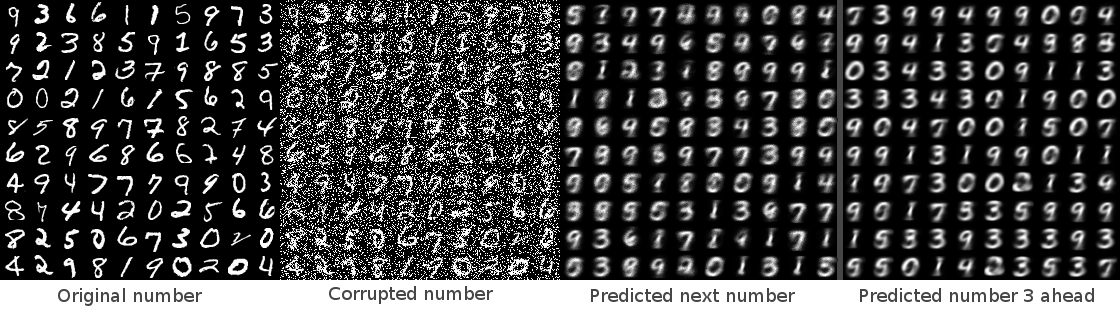
\includegraphics[width=1.0\textwidth]{story2_reconstruction}
\caption{Untied GSN reconstruction of predicted next digits and predicted digits 3 iterations ahead after 300 iterations.}
\end{figure}

Learning with untied weights is much slower, but still provides evidence that the hidden layers themselves can learn useful representations for complex input sequences. Looking at the generated samples in Figure 6.2 after 300 training iterations, mixing between sequential modes is evident as the samples appear to be generated in the same 0-9 order as the sequenced data.

\begin{figure}[h!]
  \centering
    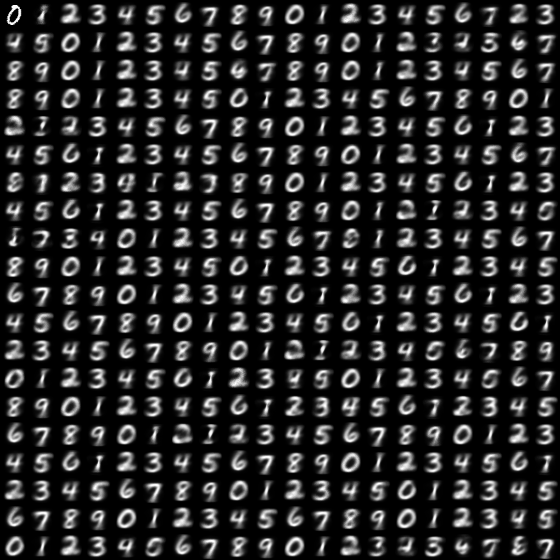
\includegraphics[width=.8\textwidth]{story2_samples_300}
\caption{Untied GSN sampling after 300 iterations.}
\end{figure}

The quality of images shown here encourage the use of separate parameters to decouple sequential learning from input representation learning.

\section{Extending the walkback procedure to sequenced inputs}

This online model loses the ability to use walkback training to reduce spurious modes. However, walkback could be generalized to the sequential case by sampling from possible variations of past hidden representations that could lead to the current input. Intuitively, this idea comes from the method of explaining current inputs with imperfect memory recall of past inputs. By sampling from the representation layer repeatedly, a series of potentially viable past representations that lead to the current input are created and used to train GSN parameters leading to the current input. This method uses past inputs as context to create viable variations of sequences in the representation space, which in turn acts to create more robust mixing between the modes in the sequence space.

The general process for creating sequential walkbacks described here is as follows:
\begin{algorithm}[h!]
	\For{k walkbacks}{
		Given input \(x\), take a backward step with the GSN using transposed weights and negated bias to create the previous hidden representation \(H\)\;
		Sample from the hidden representation \(H\) to form \(H'\)\;
		Take a forward step with the GSN using \(H'\) to create \(x'\)\;
		Use this \((x', x)\) pair as a training example for the GSN parameters\;
	}
	\caption{ Walkbacks for sequential input }
\end{algorithm}

\section{RNN-GSN: Generalizing the EM training model for the TGSN}

\begin{figure}[h!]
  \centering
    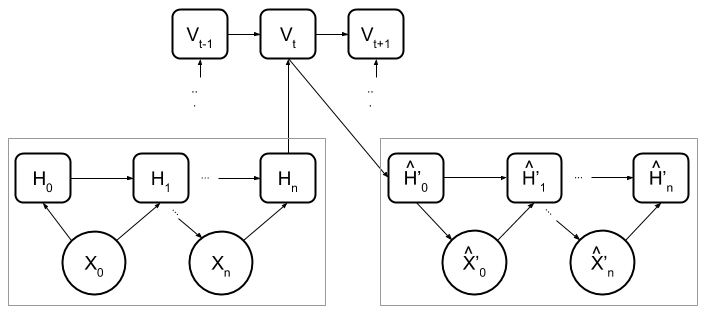
\includegraphics[width=0.8\textwidth]{rnngsn_arch}
\caption{Recurrent GSN architecture. H is GSN hiddens, V is RNN hiddens.}
\end{figure}

The EM model is easier to train and appears to have better mixing in both the input and sequence spaces compared to the online learning model. However, due to the simple regression step, it is unable to represent complex sequences in the representation space. A more general model is necessary to encode complex data in both input and representation spaces.

Ultimately, this model generalizes the TGSN by alternating between finding a good representation for inputs and a good representation for sequences. Instead of a direct encoding \(H_{t} \rightarrow H_{t+1}\), this model learns the encoding of \(P(H_{t+1}|H_{t}...H_{0})\) This way, the GSNs can optimize specifically for reconstruction or prediction rather than making the hidden representation learn both. Further, by making the sequence prediction GSN layer recurrent over the top layer of the input reconstruction GSN layer, this system can learn complex, nonlinear sequence representations over the modes of the input space, capturing a very large possibility of sequential data distributions. These two specified layers can then be repeated to form deep, generalized representations of sequential data.

\section{Algorithm}
This algorithm also alternates between training the reconstruction GSN parameters and prediction GSN for transitions.
 \begin{algorithm}[h!]
	\KwIn{training data \(X\) from a sequential distribution \(D\)}
	Initialize reconstruction GSN parameters \(\Theta_{gsn} = \) \{List(weights from one layer to the next), List(bias for layer))\}\;
	Initialize transition RNN parameters \(\Theta_{rnn} = \) \{List(weights from one layer to the next higher), List(weights from one layer to the next lower), List(bias for layer))\}\;
	\While{training not converged}{
		\For{each input \(X\)}{
			Sample from reconstruction GSN with walkback using \(X\) to create \((X_{recon},X)\) pairs for training parameters \(\Theta_{gsn}\)\;
			Compute RNN using the hidden representations \(H\) from the reconstruction GSN on the input \(X\)\;
			Store the predicted next hidden representations \(H'\) and use them with sampling from the next reconstruction GSN to train the transition parameters \(\Theta_{rnn}\)\;
		}
	}
	\caption{ Recurrent GSN Algorithm }
\end{algorithm}


\section{Experimental setup}
The RNN-GSN uses the same general training parameters with regards to noise, learning rate, annealing, momentum, epochs, hidden layers, and activation as the TGSN. In addition, it has one recurrent (LSTM) hidden layer of 3000 units, receiving input from layer 1 and layer 3 of the GSN below it. No sequential walkback steps were performed. The RNN-GSN performed worse with regards to binary cross-entropy of the predicted reconstruction than the TGSN (achieving a score of 0.2695, with the current reconstruction achieving a score of 0.1669). However, the reconstruction and predicted reconstruction after 300 training iterations qualitatively looks like the model is learning the correct sequence. Further, because of the additional recurrent layer and parameters, this model should take longer to train and slower progress to sequence prediction is expected. Further study of this general model should be with hyper-parameter optimization and more training epochs.

\begin{figure}[h!]
  \centering
    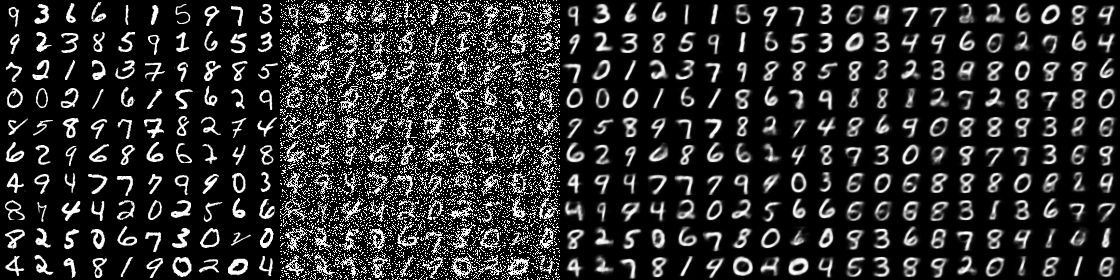
\includegraphics[width=1.0\textwidth]{story3_reconstruction}
\caption{RNN-GSN reconstruction of current digits and predicted next digits after 300 iterations.}
\end{figure}

\begin{figure}[h!]
  \centering
    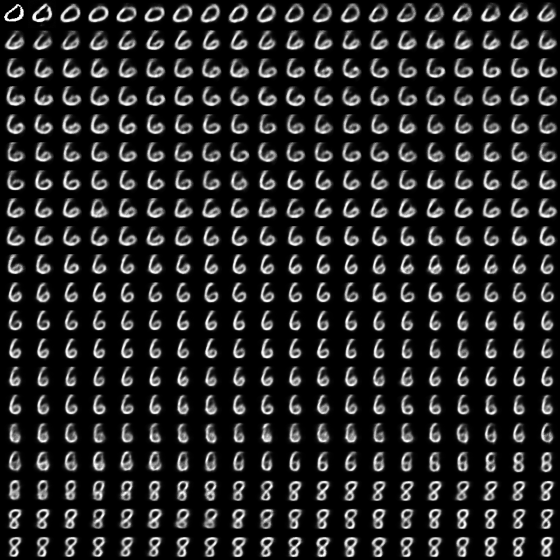
\includegraphics[width=.8\textwidth]{story3_samples_170}
\caption{RNN-GSN sampling after 300 iterations.}
\end{figure}